\begin{example}
רוצים למצוא (ולהדפיס) את כל קבצי התמונות ששמורות על הכונן הקשיח.
\end{example}
למשל עבור:
\begin{center}
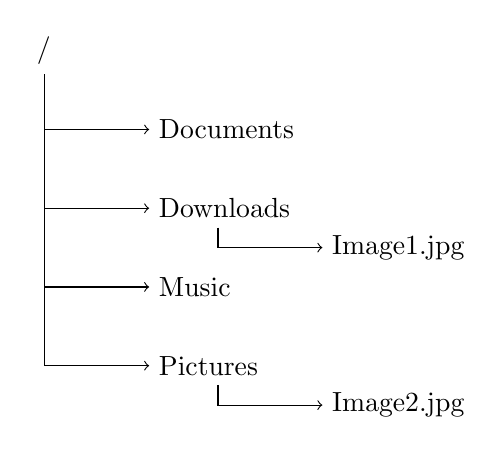
\begin{tikzpicture}[every node/.style={
	rectangle
%	, minimum width=1.5cm
%	, draw
	, text width=1.5cm
	, x=2.2cm
}, ->]

\node[text width=2mm](0) at(0,1) {/};
\foreach [count=\i] \x \y \name in {
	1/0/Documents
	, 1/-1/Downloads
	, 1/-2/Music
	, 1/-3/Pictures
	, 2/-1.5/Image1.jpg
	, 2/-3.5/Image2.jpg	
}{
	\node(\i) at(\x, \y) {\name};
}

\foreach \i in {1,...,4}{
	\draw (0) |- (\i);
}
\draw (2) |- (5);
\draw (4) |- (6);

\end{tikzpicture}
\end{center}

כיצד עלינו לסרוק (לחפש) את מערכת הקבצים ? 
\begin{enumerate}
\item
במידה ורוצים להדפיס את (הנתיב המלא של) הקבצים בסדר לקסיקוגרפי ?
\item
במידה ורוצים להדפיס קבצים לפי העומק שלהם (מספר תיקיות) ?
\end{enumerate}
נשים לב שאפשר לייצג את מערכת הקבצים באמצעות גרף מכוון (ברוב מערכות הקבצים עץ אינו ייצוג מספק)
ולכן נעביר את הדיון שלנו לחיפוש בגרפים.


